%%%%%%%%%%%%%%%%%%%%%%%%%%%%%%%%%%%%%%%%%%%%%%%%%%%%%%%%%%%%%%%%%%%%%%%%%%%%%%%
\section{Methodology}
\label{sec:methodology}
%%%%%%%%%%%%%%%%%%%%%%%%%%%%%%%%%%%%%%%%%%%%%%%%%%%%%%%%%%%%%%%%%%%%%%%%%%%%%%%

%%%%%%%%%%%%%%%%%%%%%%%%%%%%%%%%%%%%%%%%%%%%%%%%%%%%%%%%%%%%%%%%%%%%%%%%%%%%%%%
\subsection{Continous Energy Calculations with OpenMC}
\label{subsec:openmc}

-OpenMC~\cite{romano2013openmc}
-Python API~\cite{boyd2016bigdata}
-NNDC data~\cite{nndc2016endf}
-distribcell tallies~\cite{lax2014distribcell}
-\texttt{openmc.mgxs}
  -tallied in CASMO's seventy energy group structure~\cite{rhodes2006casmo}
-iso-in-lab
-runtime parameters:
  -num. particles, batches
  -computer hardware

%%%%%%%%%%%%%%%%%%%%%%%%%%%%%%%%%%%%%%%%%%%%%%%%%%%%%%%%%%%%%%%%%%%%%%%%%%%%%%%
\subsection{Multi-Group Calculations with OpenMOC}
\label{subsec:openmoc}

-OpenMOC~\cite{boyd2014openmoc}
-multi-core parallelism~\cite{boyd2016parallel}
-runtime parameters:
  -azim angles, spacing
  -num. FSRs
  -CMFD energy and spatial mesh
  -computer hardware


%%%%%%%%%%%%%%%%%%%%%%%%%%%%%%%%%%%%%%%%%%%%%%%%%%%%%%%%%%%%%%%%%%%%%%%%%%%%%%%
\subsection{Pin-wise Spatial Homogenization Schemes}
\label{subsec:homogenize}

-from Sec. 8.2
-focus less on introducing these as ``schemes'' per se
  -rather two spatial self-shielding models to quantify approx. error

%%%%%%%%%%%%%%%%%%%%%%%%%%%%%%%%%%%%%%%%%%%%%%%%%%%%%%%%%%%%%%%%%%%%%%%%%%%%%%%
\subsubsection{Null Homogenization}
\label{subsubsec:homogenize-null}

-from Sec. 8.2.2

%%%%%%%%%%%%%%%%%%%%%%%%%%%%%%%%%%%%%%%%%%%%%%%%%%%%%%%%%%%%%%%%%%%%%%%%%%%%%%%
\subsubsection{Degenerate Homogenization}
\label{subsubsec:homogenize-degenerate}

-from Sec. 8.2.3

-OpenCG region differentiation~\cite{boyd2015opencg}

\begin{figure}[h!]
\centering
\begin{subfigure}{0.35\textwidth}
  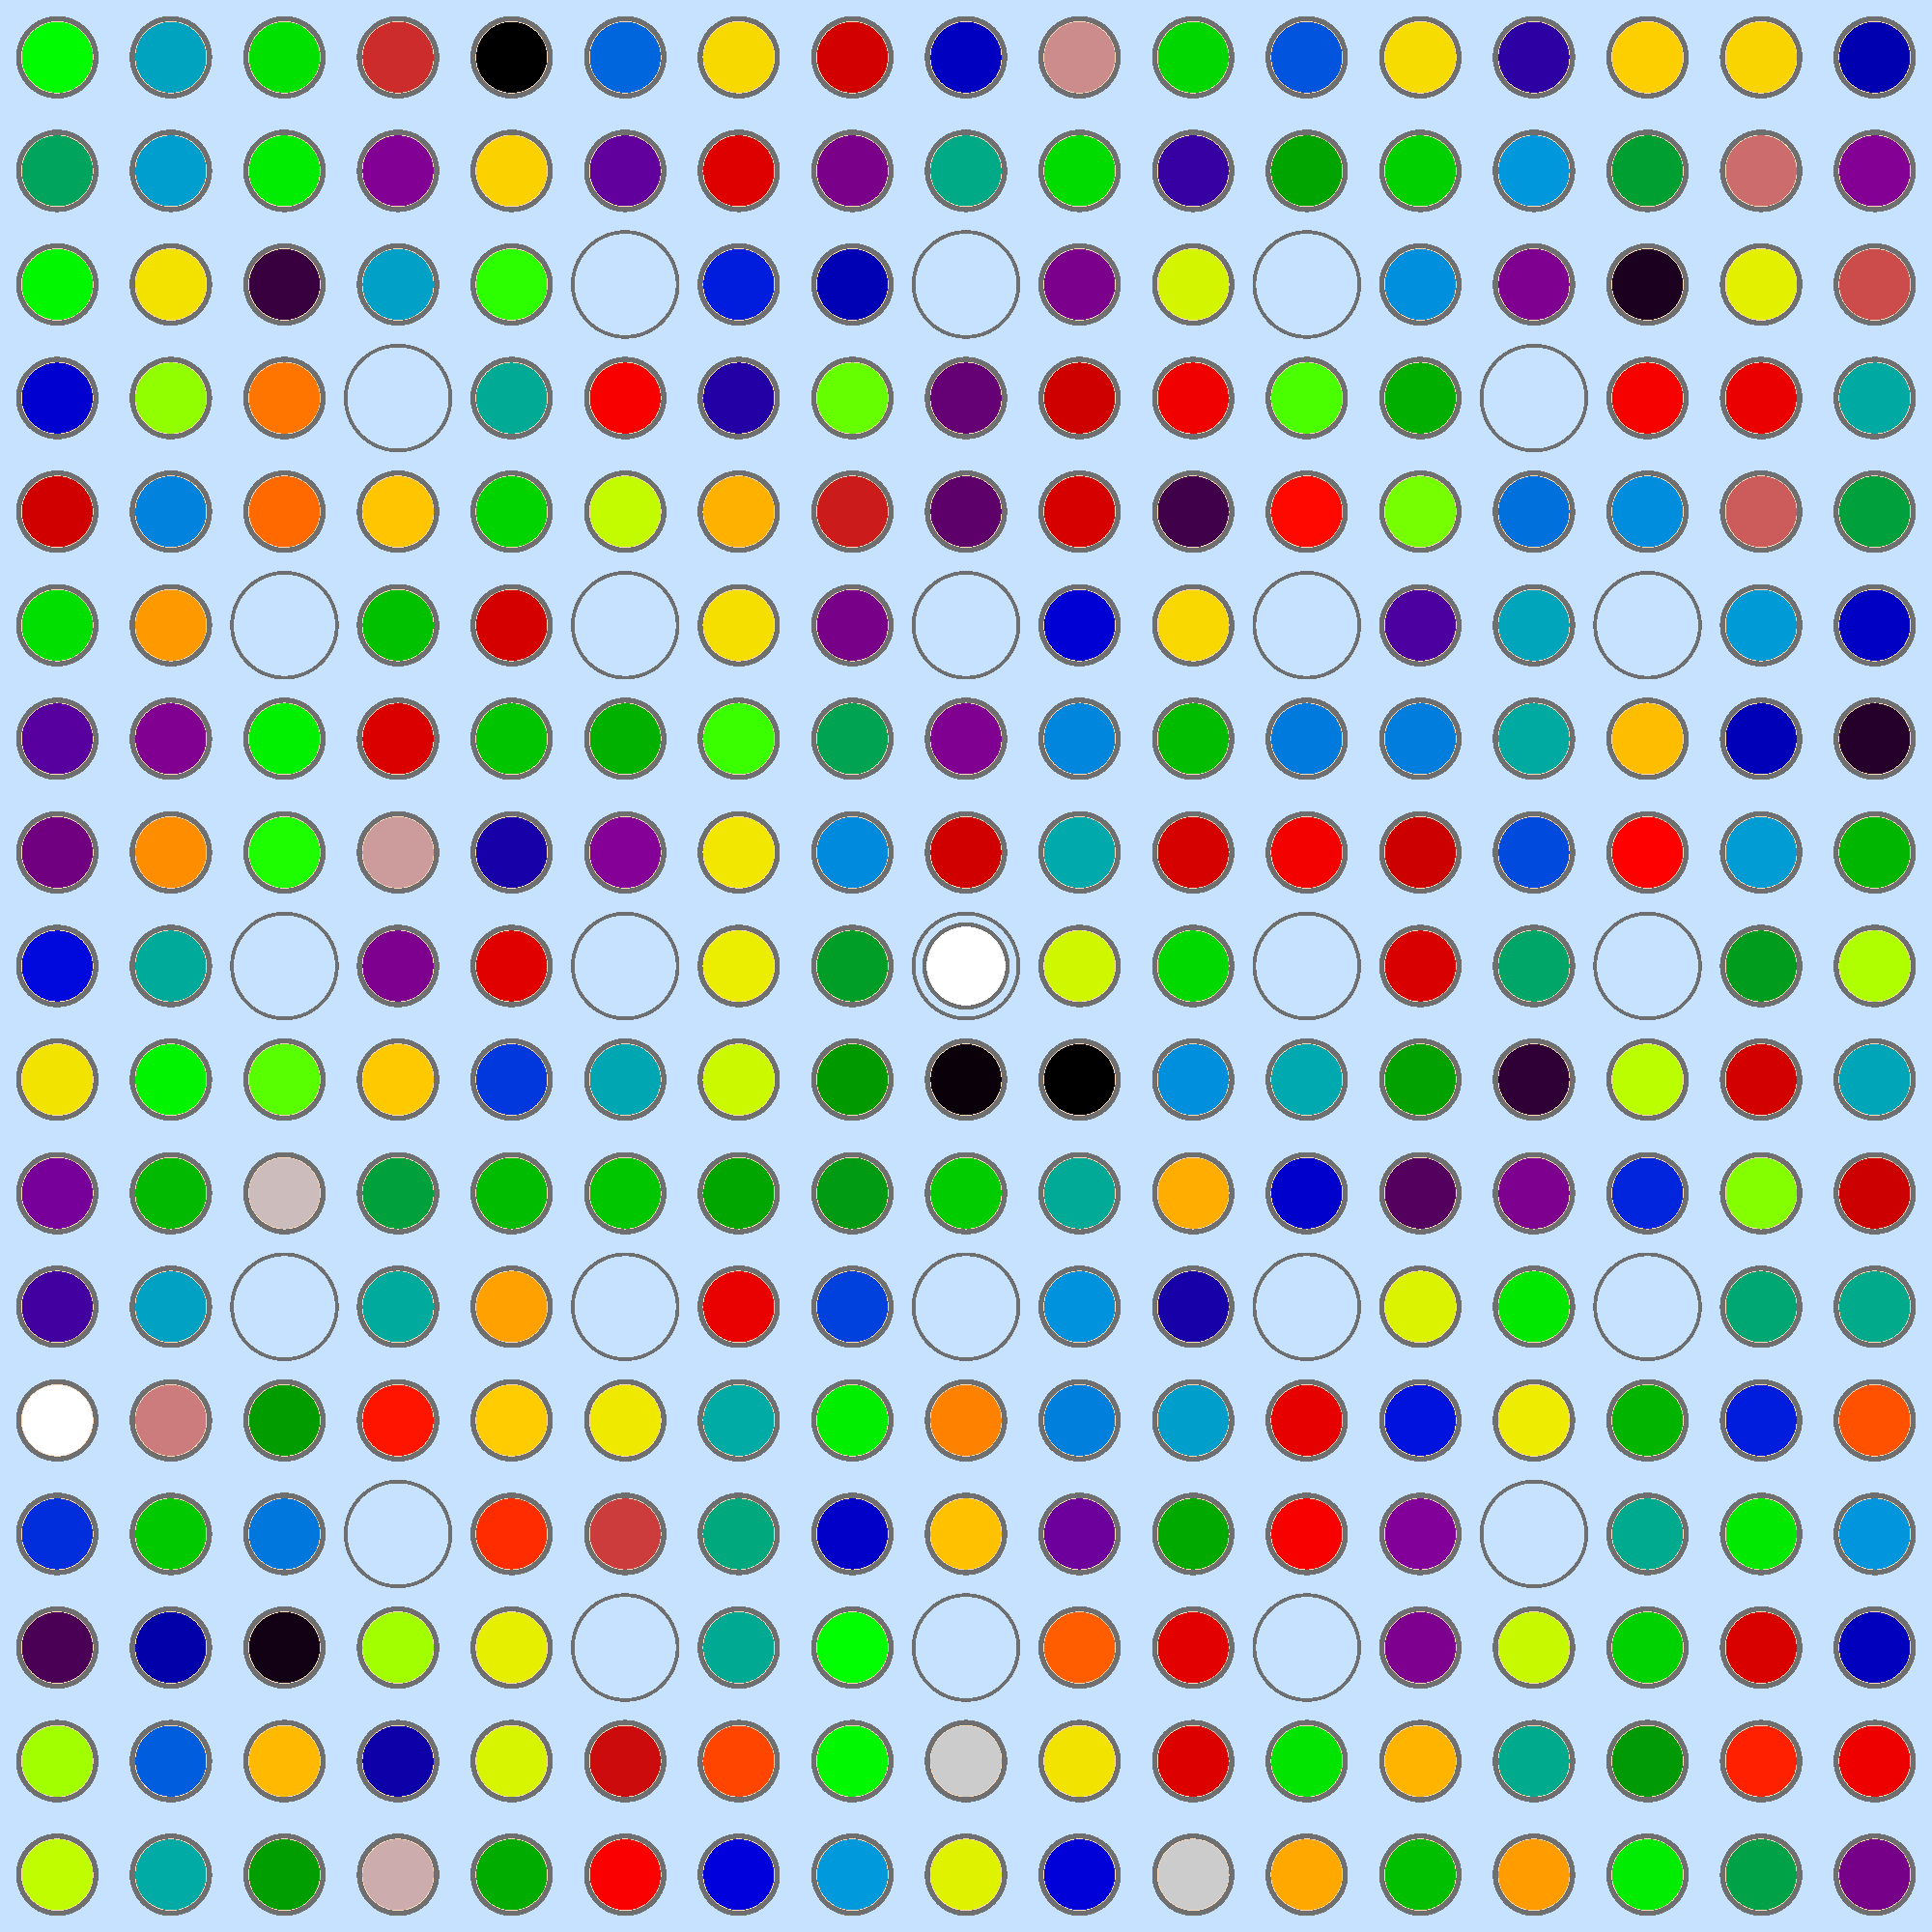
\includegraphics[width=\linewidth]{figures/assm-degen-mats}
  \caption{}
  \label{fig:degenerate-assm}
\end{subfigure}
\begin{subfigure}{0.35\textwidth}
  \centering
  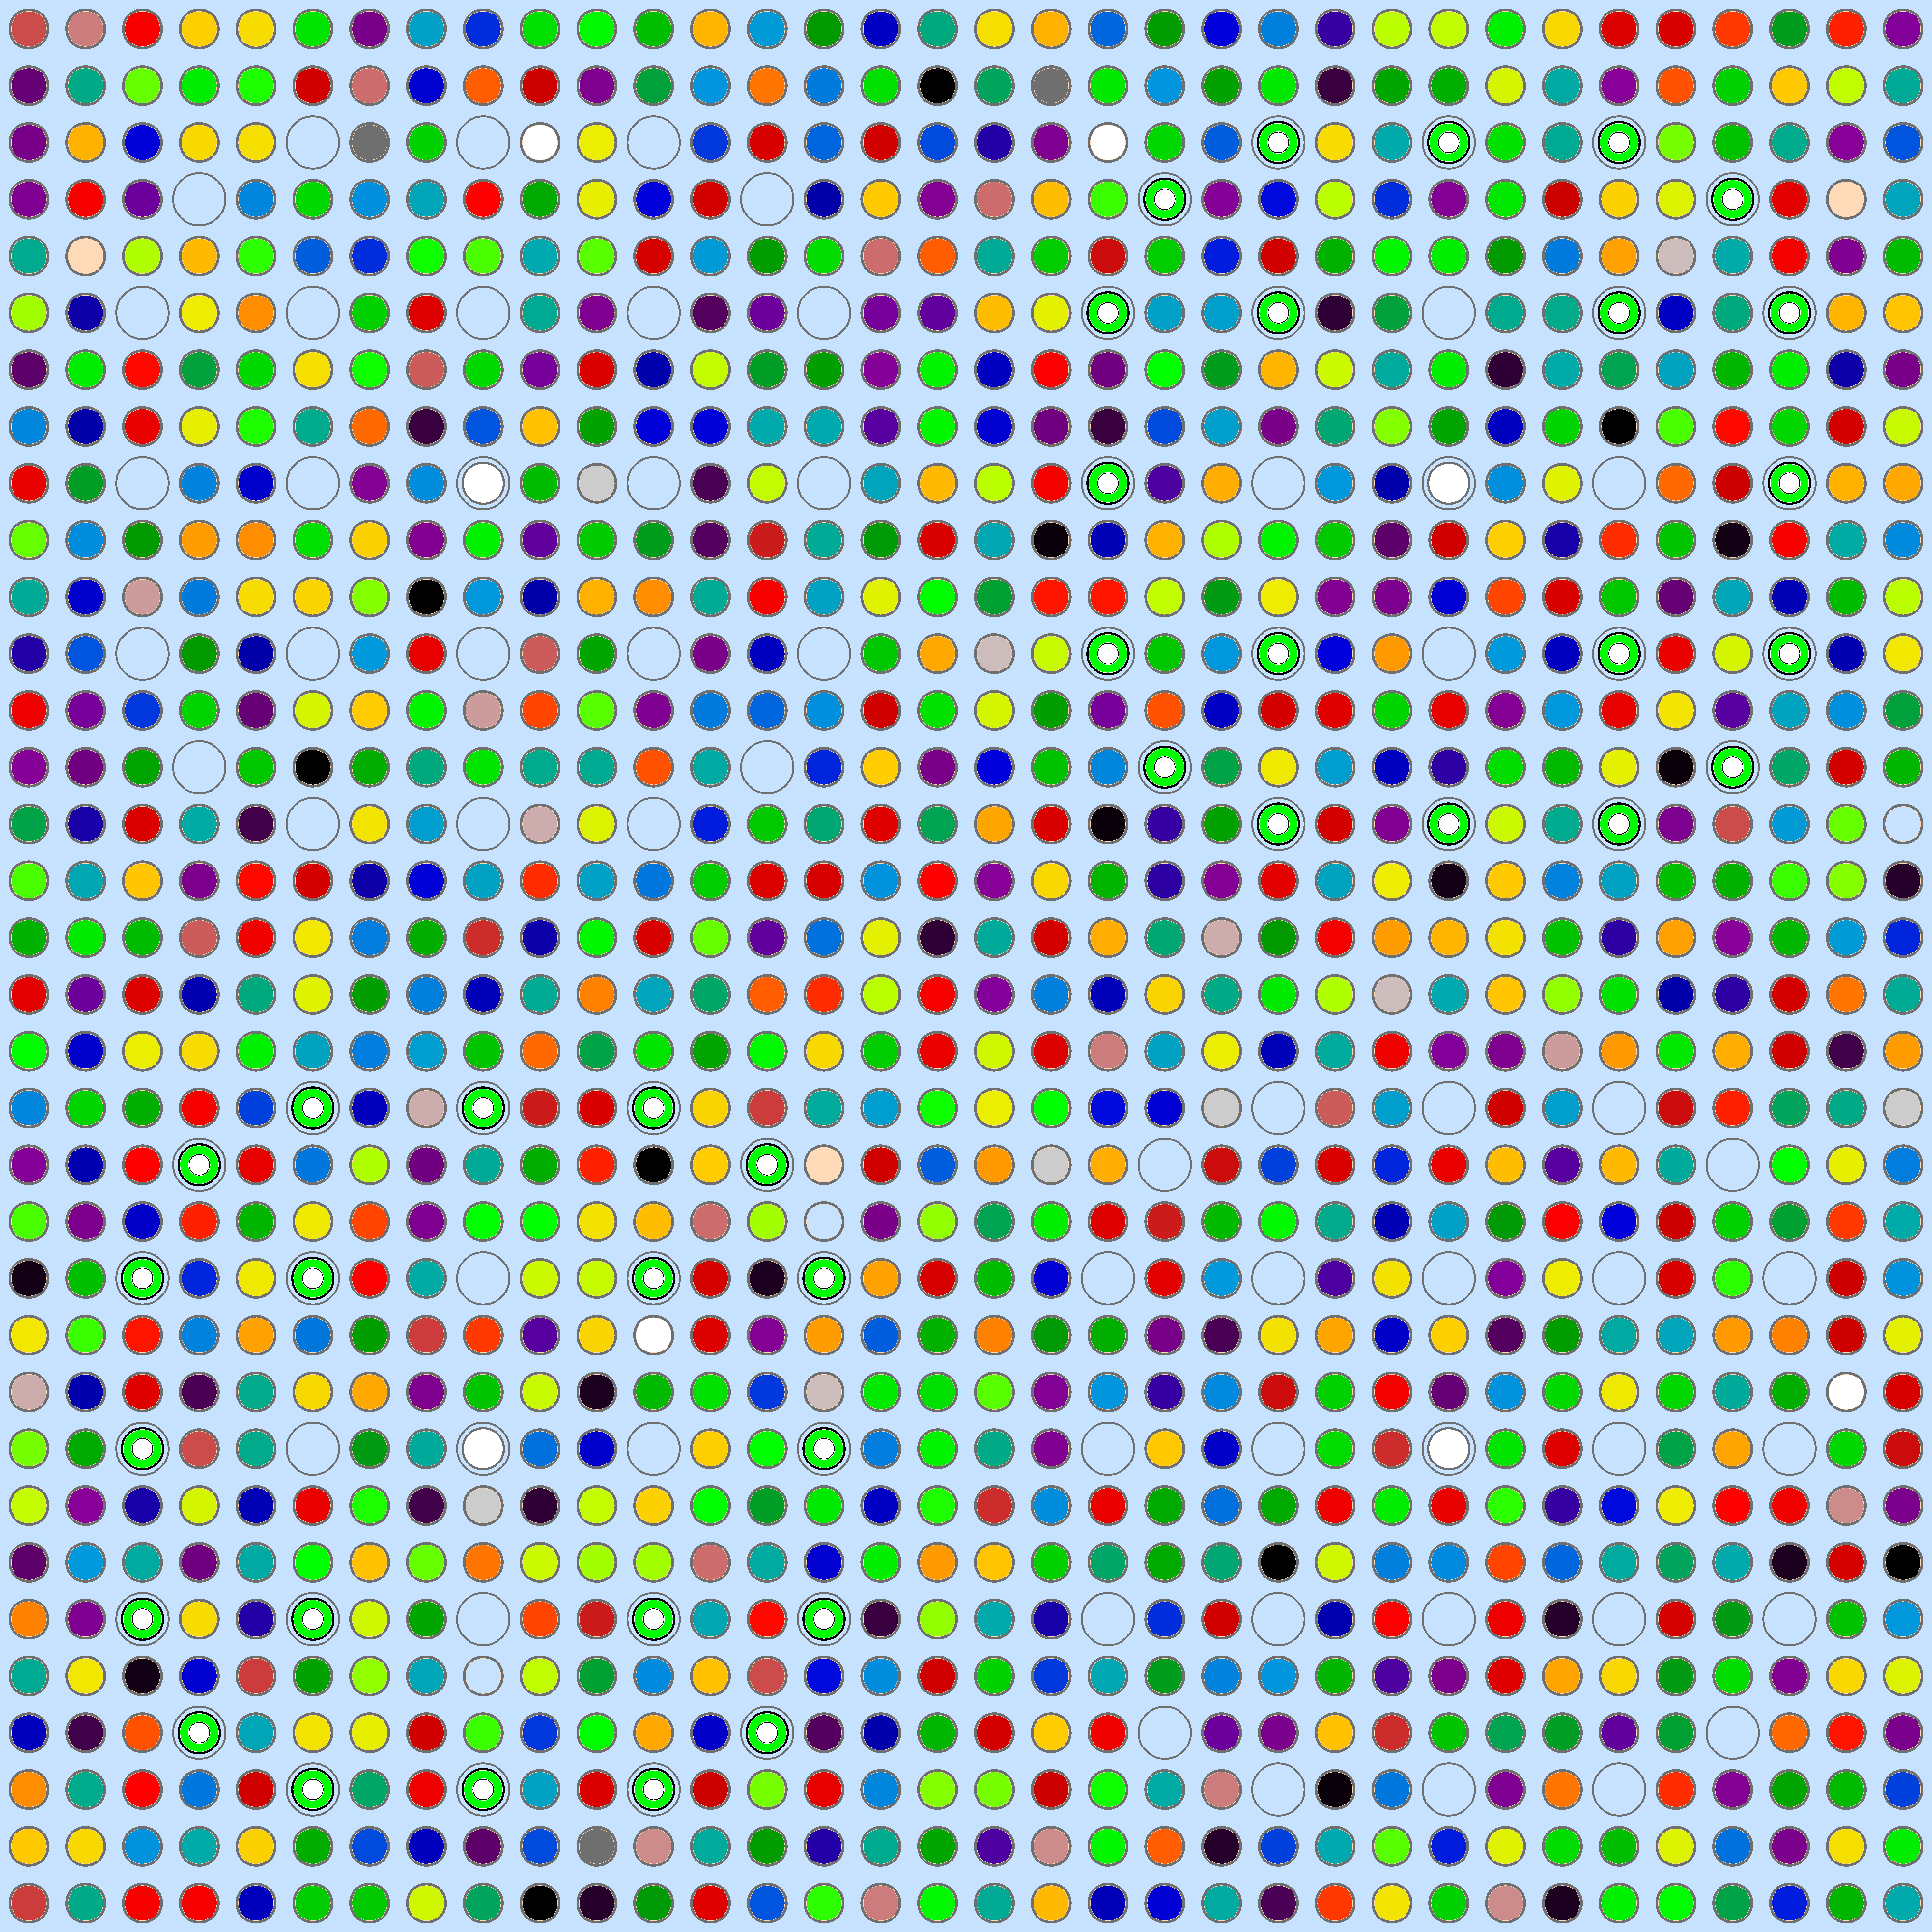
\includegraphics[width=\linewidth]{figures/reflector-degen-mats}
  \caption{}
  \label{fig:degenerate-reflector}
\end{subfigure}
\caption{OpenMOC materials for the (a) assembly and (b) 2$\times$2 colorset models with degenerate homogenization.}
\label{fig:degenerate-geometries}
\end{figure}
